%%%%%%%%%%%%%%%%%%%%%%%%%%%%%%%%%%%%%%%%%%%%%%%%%%%%%%%%%%%
%%%%%%%%%%%%%%%%%%%%%%%%%%%%%%%%%%%%%%%%%%%%%%%%%%%%%%%%%%%
\section{Extensions and Future Work}
%%%%%%%%%%%%%%%%%%%%%%%%%%%%%%%%%%%%%%%%%%%%%%%%%%%%%%%%%%%
%%%%%%%%%%%%%%%%%%%%%%%%%%%%%%%%%%%%%%%%%%%%%%%%%%%%%%%%%%%


%%%%%%%%%%%%%%%%%%%%%%%%%%%%%%%%%%%%%%%%%%%%%%%%%%%%%%%%%%%
\subsection{Geometry Makes a Comeback}
%%%%%%%%%%%%%%%%%%%%%%%%%%%%%%%%%%%%%%%%%%%%%%%%%%%%%%%%%%%

\begin{frame}[t]
%\vskip 25pt
\centering
\begin{figure}
\centering

\begin{figure}
\centering
  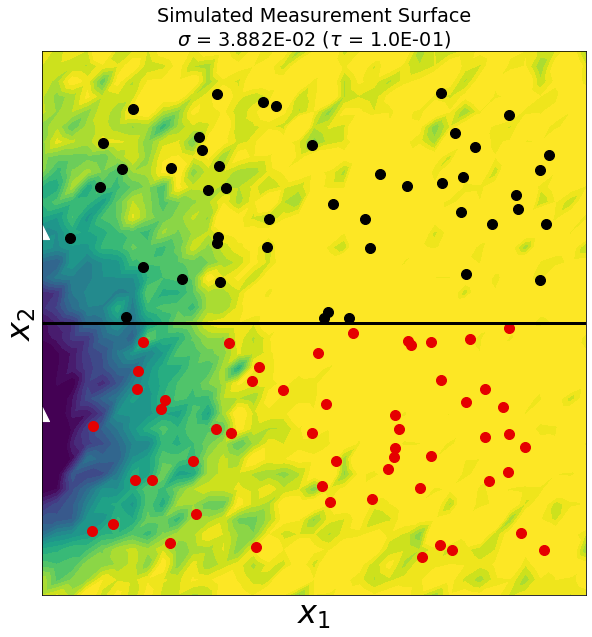
\includegraphics[width=0.25\linewidth]{figures/pde-highd_sensors_D2.png}
  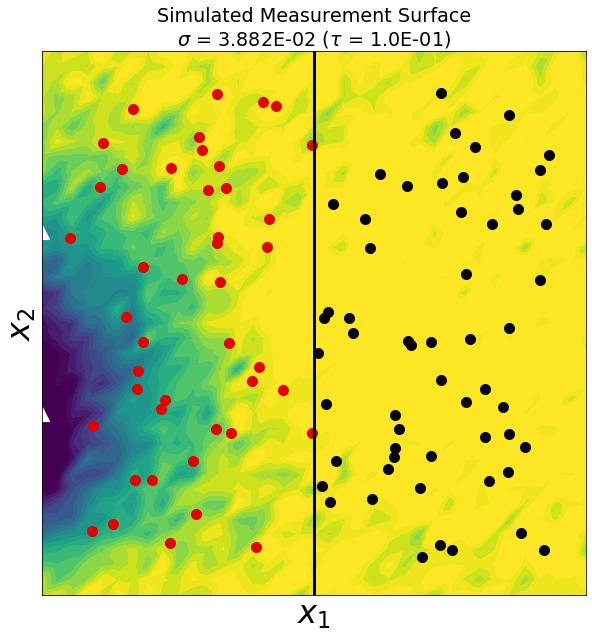
\includegraphics[width=0.25\linewidth]{figures/pde-highd_sensors-alt_D2.png}
  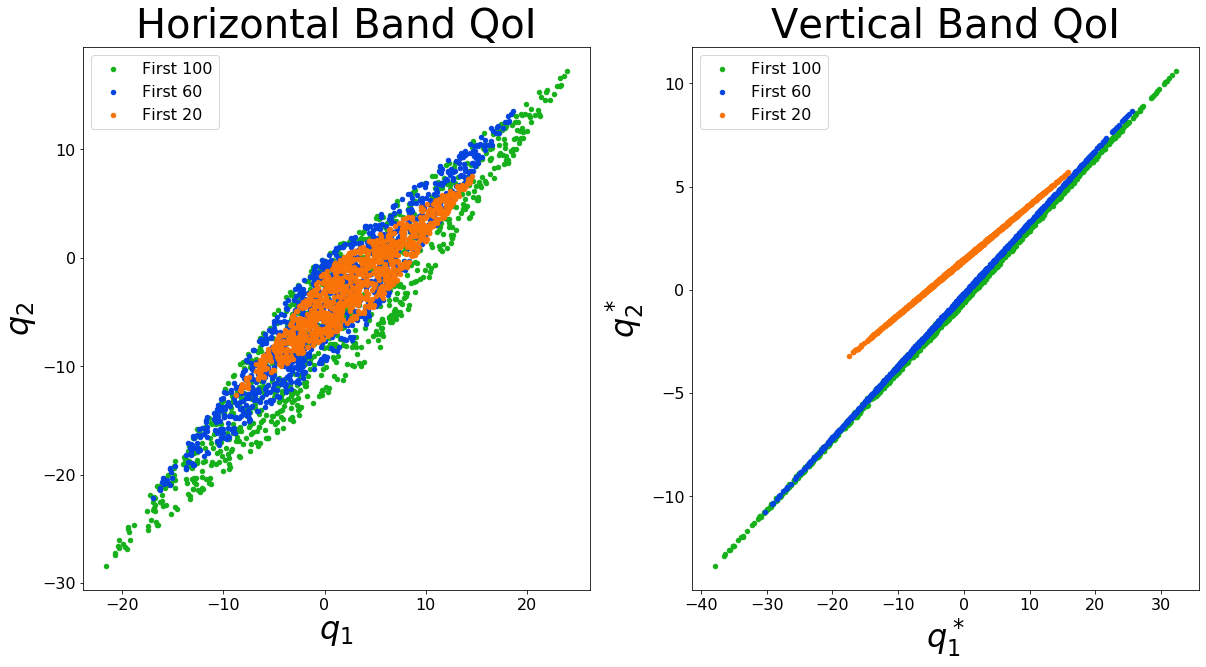
\includegraphics[width=0.5\linewidth]{figures/pde-highd_geom_D2.png}
\caption{
$N=1000$ parameter evaluations for both methods of partitioning $\Omega$.
}
\label{fig:pde-highd-2d-geometry}
\end{figure}


\end{figure}

\end{frame}


%%%%%%%%%%%%%%%%%%%%%%%%%%%%%%%%%%%%%%%%%%%%%%%%%%%%%%%%%%%
\subsection{Iterating}
%%%%%%%%%%%%%%%%%%%%%%%%%%%%%%%%%%%%%%%%%%%%%%%%%%%%%%%%%%%

\begin{frame}[t]

The one with the small problems in many batches.

\begin{figure}
  \centering
  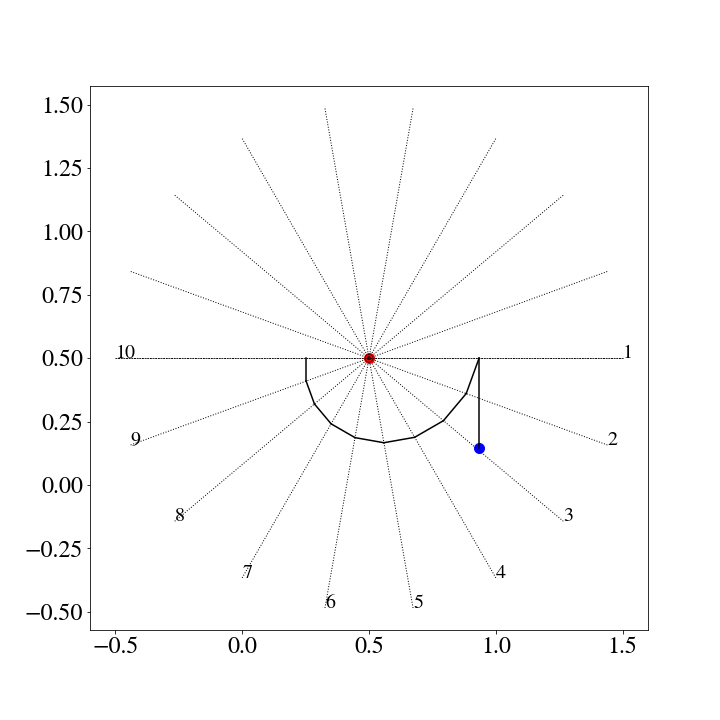
\includegraphics[width=0.475\linewidth]{figures/iterative/10D-firstepoch.png}
  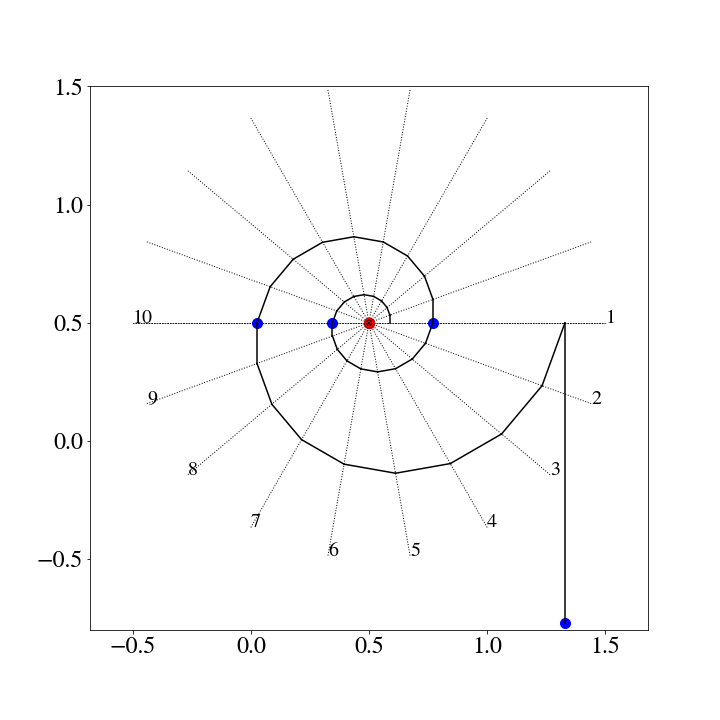
\includegraphics[width=0.475\linewidth]{figures/iterative/10D-fewepochs.png}

  \caption{
  Dotted lines show the solution contours for each row of the operator $A$.
  (Left): First epoch for iterating through 10 QoI.
  (Right): Three more epochs allows our estimate to get much closer to the true value.
  }
  \label{fig:iterative-linear-demo}
\end{figure}

\end{frame}

\begin{frame}[t]
%\vskip 25pt
\begin{figure}
\centering

\only<1>{
\begin{figure}
  \centering
  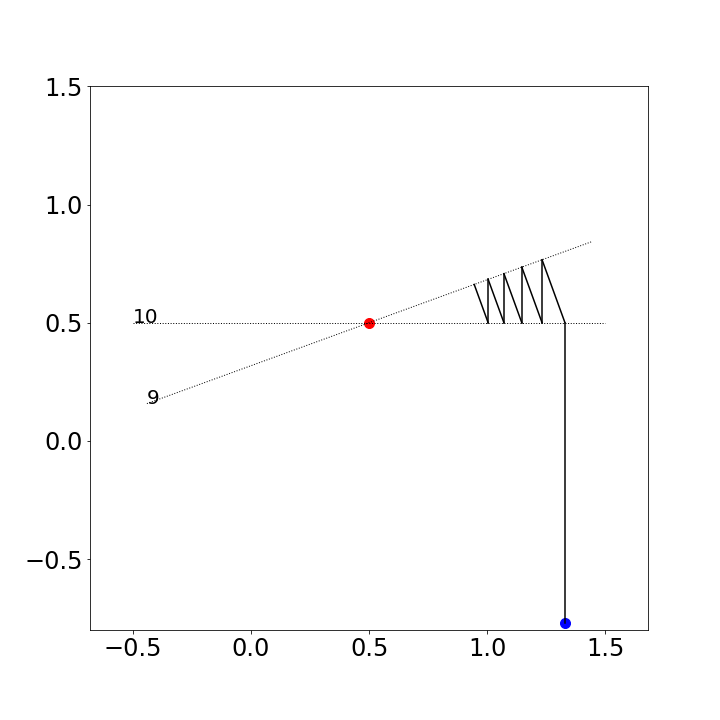
\includegraphics[width=0.475\linewidth]{figures/iterative/10D-fewepochs-pair.png}
  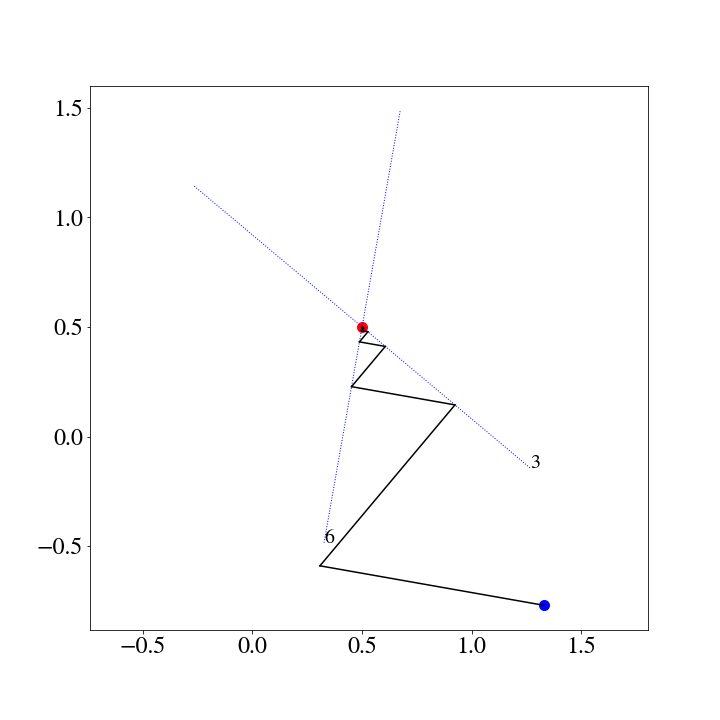
\includegraphics[width=0.475\linewidth]{figures/iterative/10D-fewepochs-pair-alt.png}
  \caption{
  Iterating through five epochs of two QoI, each formed by picking two of the ten available rows of $A$ at random.
  The random directions chosen on the left exhibit more redundancy than those on the right, so the same amount of iteration results in less accuracy.
  }
  \label{fig:iterative-linear-demo-pair}
\end{figure}
}

\only<2>{
\begin{figure}
  \centering
  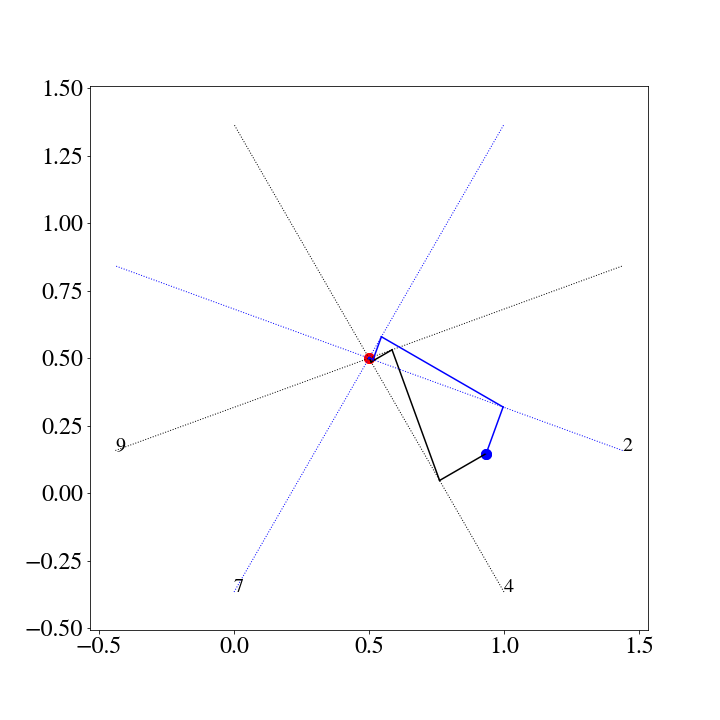
\includegraphics[width=0.475\linewidth]{figures/iterative/10D-firstepoch-pair-smart.png}
  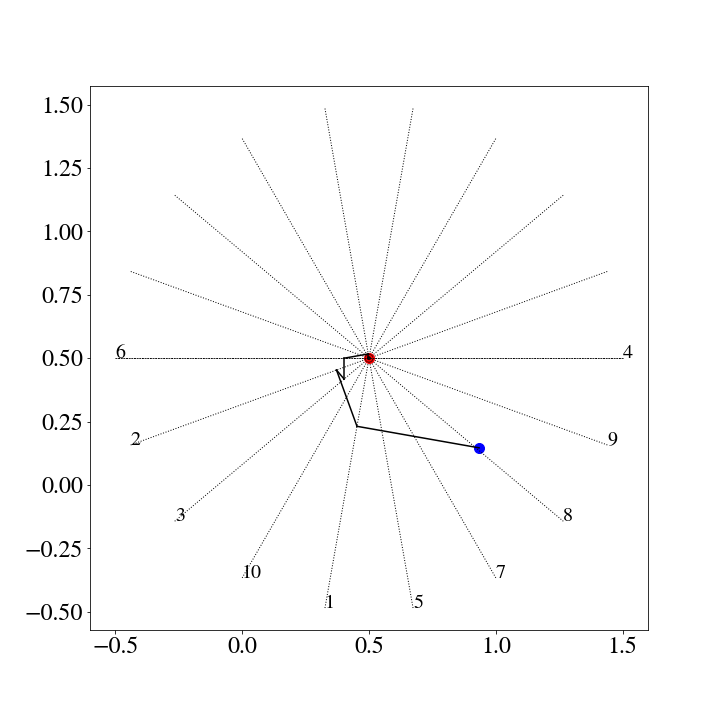
\includegraphics[width=0.475\linewidth]{figures/iterative/10D-firstepoch-rand.png}
  \caption{
  (Left): Subsets of available QoI components can be chosen to exhibit minimal redudancy and lead to expedited convergence.
  (Right): Random components of the QoI map used for each iterative step. This leads to an overall similar level of precision in this example, without the need to use gradients.
  }
  \label{fig:iterative-linear-demo-smart}
\end{figure}
}

\only<3>{
\begin{figure}
  \centering
  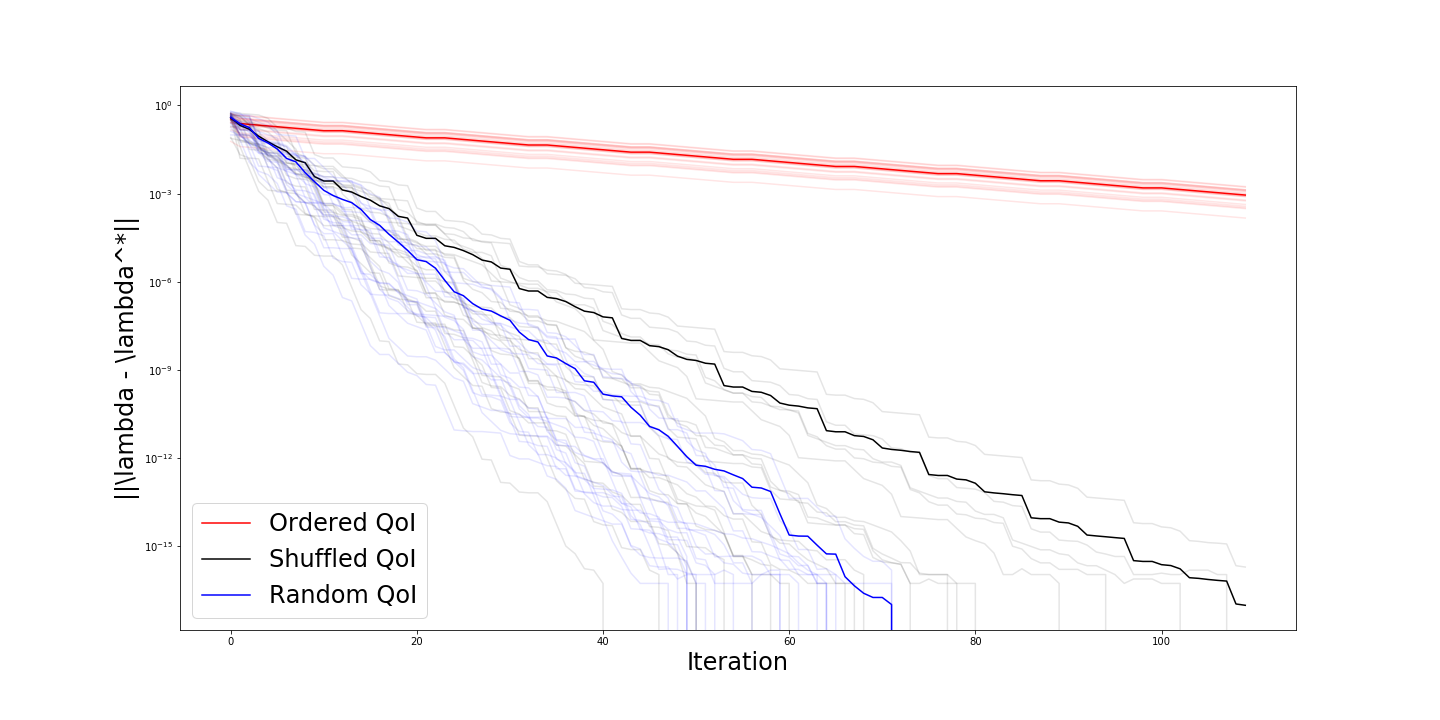
\includegraphics[width=0.95\linewidth]{figures/iterative/10D-convergence-comparison.png}
  \caption{
  20 initial means are chosen and iterated on for three approaches for ordering QoI.
  Individual experiments are transparent and the mean error is shown as a solid line for each approach.
  }
  \label{fig:iterative-convergence-comparison}
\end{figure}
}


\end{figure}
\end{frame}


%%%%%%%%%%%%%%%%%%%%%%%%%%%%%%%%%%%%%%%%%%%%%%%%%%%%%%%%%%%
\subsection{Software}
%%%%%%%%%%%%%%%%%%%%%%%%%%%%%%%%%%%%%%%%%%%%%%%%%%%%%%%%%%%

\begin{frame}[t]
%\vskip 25pt
\centering
\begin{figure}
\centering

\emph{How do I know I can trust you?}

\vspace{0.25in}

You don't. But I enabled you to check for yourself.

\vspace{0.25in}

\begin{itemize}
	\item Public repository hosted on Github.com ({\tt github.com/mathematicalmichael/thesis})
	\item Github Actions implements Continuous Integration / Deployment
	\item Each change is validated for reproducibility
	\item {\tt makefile} for convenience ({\tt make <filename>})
	\begin{itemize}
		\item dissertation + presentation (\LaTeX, themes, style files)
		\item every example, convergence result (Python)
		\item every image in every figure
	\end{itemize}
	\item PyPi published implementation of main methods: {\tt pip install mud}
	\item Unit tests aid in ensuring integrity of functions
	\item Docker guarantees software runtime (ran on {\tt x86} and {\tt arm}) \\ {\tt docker pull mathematicalmichael/python:thesis}({\tt latex:thesis})
\end{itemize}

\end{figure}

\end{frame}

